
\section{Coherent sheaves on scheme}
\subsection{sheaves of modules}

\begin{screen}
\begin{dfn}
 $(X, O_X)$をringed spaceとする.$X$上のアーベル群の層$\mathcal{F}$が$O_X$-加群であるとは,
 \begin{itemize}
   \item $X$の任意のopen set $U$に対し,$F(U)$は$O_X(U)$加群となる.
   \item $V \subset U$に対し,以下となる.

   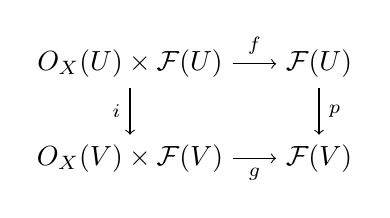
\begin{tikzpicture}[auto]
   \node (a) at (0, 1.2) {$O_X(U) \times \mathcal{F}(U)$};
   \node (x) at (2.4, 1.2) {$\mathcal{F}(U)$};
   \node (b) at (0, 0) {$O_X(V) \times \mathcal{F}(V)$};   \node (y) at (2.4, 0) {$\mathcal{F}(V)$};
   \draw[->] (a) to node {$\scriptstyle f$} (x);
   \draw[->] (x) to node {$\scriptstyle p$} (y);
   \draw[->] (a) to node[swap] {$\scriptstyle i$} (b);
   \draw[->] (b) to node[swap] {$\scriptstyle g$} (y);
   \end{tikzpicture}
 \end{itemize}
\end{dfn}
\end{screen}


この時,$\mathcal{F},\mathcal{G}$のテンソル積,$\mathcal{F} \otimes_{O_X} \mathcal{G}$を
$\mathcal{F} \otimes_{O_X} \mathcal{G}(U) := \mathcal{F}(U) \otimes_{O_X(U)} \mathcal{G}(U)$とする.
これは層になる.
また$(\mathcal{F} \otimes_{O_X} \mathcal{G})_x = \mathcal{F}_x \otimes_{O_X, x} \mathcal{G}_x$となる.
これは\ref{tensor module}で示す.


\begin{lem}
\label{tensor module}
$X$上の$O_X$加群$\mathcal{F},\mathcal{G}$のテンソル積,$\mathcal{F} \otimes_{O_X} \mathcal{G}$を
$\mathcal{F} \otimes_{O_X} \mathcal{G}(U) := \mathcal{F}(U) \otimes_{O_X(U)} \mathcal{G}(U)$とすると層になる
また$(\mathcal{F} \otimes_{O_X} \mathcal{G})_x = \mathcal{F}_x \otimes_{O_X, x} \mathcal{G}_x$となる.
\end{lem}
